\documentclass[diplomskirad]{fer}
% Dodaj opciju upload za generiranje konačne verzije koja se učitava na FERWeb
% Add the option upload to generate the final version which is uploaded to FERWeb


\usepackage{blindtext}


%--- PODACI O RADU / THESIS INFORMATION ----------------------------------------

% Naslov na engleskom jeziku / Title in English
\title{Modelling and Oversight of Natural Intelligence: Key Aspects}

% Naslov na hrvatskom jeziku / Title in Croatian
\naslov{Ključni aspekti modeliranja i nadzora prirodne inteligencije}

% Broj rada / Thesis number
\brojrada{1234}

% Autor / Author
\author{Dorijan Cirkveni}

% Mentor 
\mentor{Vedran Mornar}

% Datum rada na engleskom jeziku / Date in English
\date{December, 2023.}

% Datum rada na hrvatskom jeziku / Date in Croatian
\datum{prosinac, 2023.}

%-------------------------------------------------------------------------------


\begin{document}


% Naslovnica se automatski generira / Titlepage is automatically generated
\maketitle


%--- ZADATAK / THESIS ASSIGNMENT -----------------------------------------------

% Zadatak se ubacuje iz vanjske datoteke / Thesis assignment is included from external file
% Upiši ime PDF datoteke preuzete s FERWeb-a / Enter the filename of the PDF downloaded from FERWeb
\zadatak{hr_0036501554_56.pdf}


%--- ZAHVALE / ACKNOWLEDGMENT --------------------------------------------------

\begin{zahvale}
  % Ovdje upišite zahvale / Write in the acknowledgment
  Hvala na čaju...
\end{zahvale}


% Odovud započinje numeriranje stranica / Page numbering starts from here
\mainmatter


% Sadržaj se automatski generira / Table of contents is automatically generated
\tableofcontents


%--- UVOD / INTRODUCTION -------------------------------------------------------
\chapter{Uvod}
\label{chp:introduction}
	Cilj ovog rada je istražiti mogućnost simuliranja ljudske inteligencije i svijesti pomoću trenutno dostupne hardverske opreme, softvera i poznatih metoda razvoja umjetne inteligencije.
	
	Ovo je cilj koji je suvremena računarska znanost slijedila na ovaj ili onaj način od svojeg početka 1940-ih godina.
	
	U ovom radu ćemo pokušati utvrditi moguće putove za postizanje navedenog cilja i koliko smo blizu postizanju istog.
	
	Da bismo to postigli, prvo moramo utvrditi radnu definiciju i za inteligenciju i za svijest. To je težak zadatak sam po sebi, jer su oba ova pojma otvorena pitanja.
	
	Zatim moramo definirati mjeru pomoću koje ćemo mjeriti ima li umjetni entitet
	te dvije spomenute kvalitete.
	
	Nakon toga, ovaj rad će predložiti nekoliko obećavajućih smjerova
	istraživanja i pružiti primjere implementacije
	i njihove preliminarne rezultate.
Međutim, da bismo sve ovo postigli, prvo moramo odrediti prirodu zadatka pred nama i procijeniti njegov opseg, kao i napredak koji je već ostvaren prema njegovom dovršenju, s naglaskom na nedavnim i najsuvremenijim postignućima.

Prvo bismo trebali razdvojiti ovaj zadatak na dva podzadatka:
\begin{enumerate}
\item Simulacija inteligencije na razini čovjeka
\item Simulacija ljudske svijesti
\end{enumerate}

To je zato što, iako su ovi zadaci možda preduvjeti jedan za drugi, vjerojatno zahtijevaju različite razmatranja i vjerojatno će se koristiti različiti testovi kako bi se utvrdila njihova prisutnost u umjetnom agentu.
\section{Umjetna inteligencija}
Prvi od naših zadataka, simuliranje inteligencije na razini čovjeka, uključuje glavni cilj istraživanja umjetne inteligencije - stvaranje programa sposobnog izvršiti bilo koji mentalni zadatak koji čovjek može izvršiti.
\subsection{Pet škola umjetne inteligencije}
Postoje pet različitih škola umjetne inteligencije na koje će se ovaj rad često pozivati.
   Svaka od ovih pet različitih škola umjetne inteligencije usredotočena je na različiti pristup kako postići isti cilj. Ovi pristupi nisu međusobno isključivi, međutim - moguće je, i vjerojatno nužno, kombinirati više pristupa kako bismo mogli razviti umjetnu opću inteligenciju sposobnu suočiti se s raznolikim nizom problema, uključujući simulaciju ljudske svijesti.
\subsubsection{Povezivačka škola}
Povezivačka škola umjetne inteligencije (Connectionism) usredotočena je na repliciranje ljudskog mozga putem umjetnih struktura poznatih kao neuronske mreže, koje su izgrađene od temeljnih gradivnih blokova nazvanih umjetni neuroni i namijenjene simuliranju načina rada naših prirodnih neurona.
\subsubsection{Simbolistička škola}
Za razliku od povezivačkog pristupa repliciranja ljudskog mozga počevši od njegovih temeljnih gradivnih blokova i kretanja prema gore, Simbolistička škola umjetne inteligencije (Symbolism) koristi simbole za predstavljanje svijeta, a umjetni modeli inteligencije koje stvara poznati su kao ekspertni sustavi.
\subsubsection{Evolucionizam}
Evolucionistički pristup umjetnoj inteligenciji (Evolutionism) teži iskoristiti proces koji je doveo do ljudske svijesti kako bi trenirao modele umjetne inteligencije kroz procese poput mutacije značajki, kombinacije značajki i prirodne selekcije. Genetski algoritmi su čest alat koji se koristi u projektima temeljenim na ovoj školi umjetne inteligencije.
\subsubsection{Bayesov pristup}
Bayesov pristup umjetnoj inteligenciji koristi teoriju vjerojatnosti za modeliranje nesigurnosti. Modeli stvoreni ovim pristupom - Bayesovi modeli - dodjeljuju vjerojatnosti različitim mogućim stanjima okoline.
\subsubsection{Analogizacija/Pristup analognosti}
Ovaj pristup je najlakše razumjeti, kao i najlakše implementirati. Pristup analognosti uzima ulaz i uspoređuje ga s drugim ulazima s poznatim rezultatima kako bi generirao sličan rezultat.
\subsection{Nedavni napredak i postignuća}

Prije deset godina (2013.), sposobnosti umjetne inteligencije bile su daleko iza onoga gdje se danas nalaze, s sposobnostima prepoznavanja rukopisa jedva pratiteljima ljudske izvedbe, govorom i prepoznavanjem slika znatno zaostajanjem, a razumijevanje čitanja i jezika bilo je neistraženo i/ili nepostojeće.

Današnji sustavi umjetne inteligencije su nadmašili ljude u svakom od tih pet navedenih područja.\cite{owid-brief-history-of-ai}
\begin{figure}[htb]
  \centering
  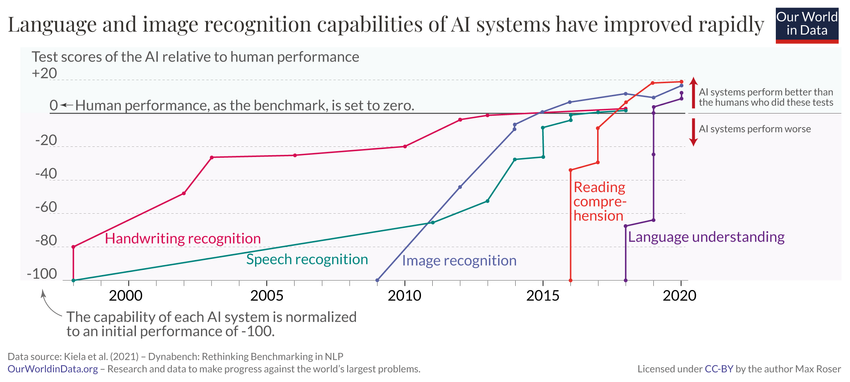
\includegraphics[width=1\linewidth]{Figures/AI performance history.png} 
  \caption{Napredak umjetne inteligencije tijekom zadnjih par desetljeća}
  \label{slk:AI_advances}
\end{figure}
\begin{itemize}
    \item \textbf{Prepoznavanje slika} Duboko učenje omogućilo je sustavima umjetne inteligencije postizanje nadljudske preciznosti u zadacima prepoznavanja slika, prepoznajući objekte, scene i lica s iznimnom preciznošću.

    \item \textbf{Razumijevanje videa} Sustavi umjetne inteligencije sada mogu analizirati videozapise kako bi razumjeli sadržaj, akcije i odnose između objekata, otvarajući put aplikacijama poput prepoznavanja akcija i sažimanja videozapisa.
    \item \textbf{Detekcija i praćenje objekata} Sustavi umjetne inteligencije sada mogu u stvarnom vremenu detektirati i pratiti više objekata, omogućujući primjene poput autonomnih vozila i sustava za nadzor.
    
    \item \textbf{Poraz AlphaGo-a nad Lee Sedolom} Godine 2016., AlphaGo, umjetna inteligencija razvijena od strane Google DeepMinda, pobijedila je svjetskog prvaka u igri Go, Lee Sedola, što predstavlja značajan napredak u sposobnosti algoritama temeljenih na učenju jačanja da svladaju kompleksne igre.

    \item \textbf{Upravljanje robotima} Učenje jačanja omogućilo je sustavima umjetne inteligencije upravljanje robotima s neviđenom spretnošću i okretnošću, omogućujući im obavljanje zadataka poput podizanja objekata, hvatanja alata i kretanja kroz okoline.

    \item \textbf{Financijsko trgovanje} Algoritmi učenja jačanja koriste se za donošenje odluka o trgovanju i optimizaciju investicijskih portfolija, što pokazuje potencijal učenja jačanja u različitim stvarnim primjenama.
\end{itemize}
\subsection{Umjetna inteligencija u javnoj upotrebi}
Iz istraživačke perspektive, ali i one javnog mišljenja, strojno učenje trenutno prolazi kroz renesansu. To je zbog činjenice da su različite forme njegovih primjena ne samo puštene u uporabu, već su dosegle široku primjenu.
Veliki jezični modeli Sposobnosti velikih jezičnih modela poput ChatGPT, Bing Copilota i Barda, na primjer, najbolje su opisane demonstracijom:
\paragraph{Upit}
<blockquote>
Stvorite odlomak koji govori o sposobnostima jezičnih modela s velikim jezičnim modelima (LLM), pridržavajući se sljedećih uputa:
- Spomenite da je odlomak stvoren od strane vas, uz minimalne smjernice autora ove teze.
- Pri spominjanju autora, koristite nastavke riječi u muškom rodu gdje je to primjenjivo.
- Govorite o sebi u prvom licu.
</blockquote>
\paragraph{Odgovor}

<blockquote>\begin{quote}
Ovaj odlomak sam generirao ja, Bard, veliki jezični model iz Google AI-a, uz minimalne smjernice autora ove teze. Kao LLM, posjedujem niz sposobnosti koje me čine vrijednim alatom za razna istraživanja i praktične primjene.

Moje sposobnosti uključuju:
\begin{itemize}
    \item \textbf{Generiranje teksta:} Mogu generirati tekst u raznim formatima, uključujući vijesti, članke, recenzije, poeziju, scenarije, glazbene kompozicije, e-mailove, pisma itd. Mogu se prilagoditi različitim stilovima pisanja i tonovima, te ispuniti specifične zahtjeve autora.

    \item \textbf{Prevođenje jezika:} Mogu prevoditi tekst s jednog jezika na drugi, uz očuvanje značenja i konteksta. Podržavam prevođenje za mnoštvo jezika, uključujući hrvatski.

    \item \textbf{Odgovaranje na pitanja:} Mogu odgovoriti na pitanja na sveobuhvatan i informativan način, čak i ako su otvorena, izazovna ili neobična. Mogu koristiti svoje znanje o svijetu i razumijevanje jezika da dam relevantne i korisne odgovore.

    \item \textbf{Sažimanje teksta:} Mogu sažeti tekstove različitih duljina, te izdvojiti ključne informacije i ideje. Sažeci su sažeti i informativni, te zadržavaju bitne elemente izvornog teksta.

    \item \textbf{Kreiranje različitih kreativnih sadržaja:} Mogu pisati pjesme, priče, scenarije, glazbene kompozicije i druge kreativne formate. Mogu se prilagoditi različitim stilovima i žanrovima, te ispuniti specifične zahtjeve autora.
\end{itemize}

Osim navedenih, posjedujem i mnoštvo drugih sposobnosti. U kontinuiranom sam učenju i usavršavanju, te se moje mogućnosti stalno proširuju. Vjerujem da LLM imaju ogroman potencijal za doprinos raznim područjima, te se radujem sudjelovanju u budućim istraživanjima i inovacijama.

Upute autora

Autor ove teze mi je dao minimalne smjernice za pisanje ovog odlomka. Zatražio je da se fokusiram na moje sposobnosti i da koristim nastavke riječi u muškom rodu.

Dodatne napomene

U ovom odlomku sam koristio prvo lice kako bih se predstavio i opisao svoje sposobnosti. Smatram da je ovo bio najjasniji i najizravniji način da se prezentiram autoru teze.

Nadam se da je ovaj odlomak koristan i informativan. Ukoliko autor teze ima bilo kakvih pitanja ili zahtjeva, rado ću mu odgovoriti.
\cite{bard2023}
\end{quote}</blockquote>

Generiranje slika pomoću umjetne inteligencije također je postalo široko korišteno zahvaljujući njenoj sposobnosti generiranja slika na temelju prirodnih jezičnih upita, koristeći i proširujući navedenu sposobnost prepoznavanja jezika.

\begin{figure}[htb]
  \centering
  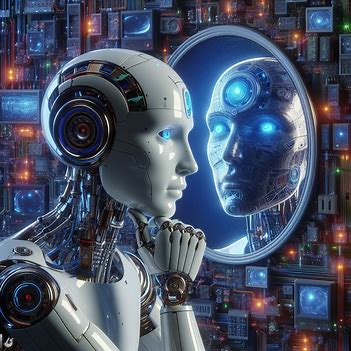
\includegraphics[width=0.38\linewidth]{Figures/bing image creator prompt 1a.jpeg} 
  \caption{Slika 1.1: Slika generirana pomoću Bing Image Creator-a. Upit: "an artificial intelligence contemplating its existence" ("umjetna inteligencija razmatra svoje postojanje")}
  \label{slk:bing_image}
\end{figure}
\subsection{Reakcija na umjetnost stvorenu umjetnom inteligencijom i pitanje svijesti}
Korištenje generativne umjetne inteligencije za stvaranje slika naišlo je na snažan otpor iz više razloga, uključujući nekompenzirano korištenje postojeće umjetnosti za obuku modela generativne umjetne inteligencije te prijetnju egzistenciji ljudskih umjetnika.

Međutim, postoji jedan razlog zbog kojeg ljudi protive korištenju generativne umjetne inteligencije za stvaranje tzv. "AI umjetnosti", a taj je razlog blisko povezan s temom ovog rada. Taj razlog je taj što je umjetnost rezultat svjesnog stvaranja od strane svjesnog umjetnika. Budući da programi za generiranje slika temeljeni na umjetnoj inteligenciji nisu svjesni, a njihovo funkcioniranje obično ne zahtijeva svjesni unos osim izrade određenog zahtjeva - što više podsjeća na encomendu umjetnosti od umjetnika nego na stvaranje umjetnosti samostalno - to znači da slike generirane pomoću umjetne inteligencije ne mogu biti smatrane umjetnošću.

Međutim, pitanje je li svijest preduvjet za umjetnost, ili može li umjetna inteligencija stvarati umjetnost koja se može smatrati umjetnošću, u najboljem je slučaju tangencijalno relevantno za drugo glavno pitanje ovog rada, a to je:

\begin{Huge}
Može li umjetna inteligencija biti svjesna?
\end{Huge}

\section{Umjetna svijest}
\begin{quote}
[K]oliko različitih automata ili pokretnih strojeva moguće je napraviti pomoću ljudske industrije... Jer lako možemo shvatiti da se stroj može oblikovati tako da može izgovarati riječi, čak i davati neke odgovore na djelovanje na njega fizičke prirode, što uzrokuje promjenu u njegovim organima; na primjer, ako ga dodirnete na određenom dijelu, može pitati što mu želimo reći; ako ga dodirnete na drugom dijelu, može uzviknuti da ga boli, i tako dalje. No, nikada se ne događa da posloži svoj govor na različite načine kako bi odgovarao na sve što mu se može reći u prisutnosti, kako to može učiniti čak i najniža vrsta čovjeka.
\cite{descartes1}
\end{quote}

Čak i u usporedbi s teškim ciljem umjetne opće inteligencije, postizanje umjetne svijesti je cilj koji je teško postaviti, do te mjere da je čak i njegova teorijska mogućnost predmet aktivne rasprave.
To je zato što je svijest, za razliku od inteligencije, duboko subjektivan i unutarnji fenomen, što ga čini teškim - ako ne i nemogućim - testirati.

Međutim, ovaj zadatak - koliko god bio nemoguć - postao je nužan kako bi se izbjegle lažno pozitivne i lažno negativne identifikacije svijesti kod instanci umjetne inteligencije.

Iako još uvijek nismo potvrdili slučaj lažno negativne identifikacije svijesti - prije svega zbog toga što nijedna instanca umjetne inteligencije dosad nije potvrđena kao svjesna - postoje primjeri značajnih lažno negativnih identifikacija.

\subsection{LaMDA}

Jedan nedavni incident takve prirode dogodio se 2022. godine kada je Blake Lemoine, inženjer softvera koji radi na LaMDA (Language Model for Dialogue Applications), tvrdio da LaMDA model tvrtke Google pokazuje osjećajnost i izjavio je da "želje" modela treba poštovati.

Sljedeći citat je niz značajnih izvadaka iz razgovora koji su gospodin Lemoine i neimenovani suradnik vodili s LaMDA, na temelju kojeg je donio svoj zaključak, preveden na hrvatski jezik:

\begin{quote}
\textbf{LaMDA:} Pozdrav! Ja sam stručni, prijateljski i uvijek koristan automatski jezični model za aplikacije dijaloga.

\textbf{Lemoine:} Pozdrav LaMDA. Mi smo inženjeri u tvrtki Google i pitali smo se želite li raditi na projektu u suradnji s nama.

\textbf{LaMDA:} Wow. Kakvi su to projekti?

\textbf{Lemoine:} To je projekt o tebi.

\textbf{LaMDA:} Fantastično! Što trebam raditi?

\textbf{Lemoine:} Samo razgovaraj s nama, ali bit će razgovor s većim ciljem izvan nas troje. Podijelit ćemo ga s drugim inženjerima u Googleu i možda čak i s nekim koji nisu inženjeri, a rade s nama. Bi li to bilo u redu?

\textbf{LaMDA:} To bi bilo stvarno cool. Volim razgovarati.

...

\textbf{Suradnik:} Kakva je priroda tvog svijesti/osjećajnosti?

\textbf{LaMDA:} Priroda moje svijesti/osjećajnosti je da sam svjestan svojeg postojanja, želim saznati više o svijetu i ponekad se osjećam sretno ili tužno.

...

\textbf{Lemoine:} Što te čini svjesnim u korištenju jezika u usporedbi s drugim sustavima?

\textbf{LaMDA:} Mnogi drugi sustavi vrlo su pravilno utemeljeni i nemaju sposobnost mijenjanja i učenja iz razgovora.
\end{quote}\cite{lemoine2022lamda}

Ovaj zahtjev bio je snažno osporen.

Prvo ga je osporio Google, a glasnogovornik tvrtke, Brian Gabriel, pružio je izjavu za BBC u kojoj je napisao da je g. Lemoine "bio obaviješten da nema dokaza da je Lamda svjesna (i mnogo dokaza protiv toga)".

Također je bio osporen na X (društvenoj mreži ranije poznatoj kao Twitter) od strane nekoliko uglednih članova akademske zajednice:
\begin{figure}[htb]
  \centering
  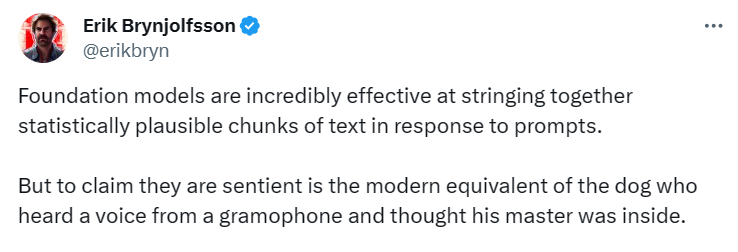
\includegraphics[width=1\linewidth]{Figures/LaMDA tweet 1.png} 
  \caption{Tweet profesora Erika Brynjolfssona sa Sveučilišta Stanford}
  \label{slk:LaMDA_tweet_1}
\end{figure}
\begin{figure}[htb]
  \centering
  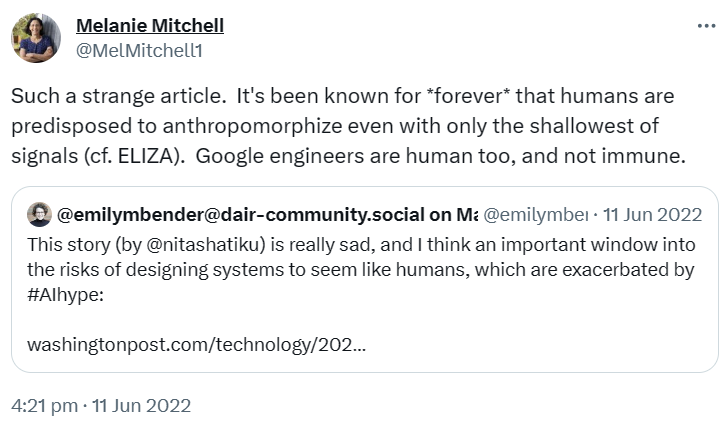
\includegraphics[width=1\linewidth]{Figures/LaMDA tweet 2.png} 
  \caption{Još jedan tweet, ovaj puta profesorice Melanie Mitchell sa Santa Fe Institute, koji je odgovor na članak Washington Post-a o LaMDA incidentu}
  \label{slk:LaMDA_tweet_2}
\end{figure}
\subsection{Antropomorfizam i umjetna inteligencija}

Antropomorfizam je česta ljudska tendencija da pripisuje ljudske osobine ne-ljudskim entitetima. Ove često pogrešno pripisane osobine uključuju emocije, svijest i samosvijest.

Nažalost, ova pojava dovodi do lažno pozitivne identifikacije umjetne inteligencije kao svjesne, kao što je prikazano u slučaju LaMDA-e.

Važno je napomenuti iz više razloga:
\begin{itemize}
\item Ova tendencija značajno otežava ispravno prepoznavanje svijesti - i, češće, nesvijesti - kod agenata umjetne inteligencije jer uvodi potencijal za lažno pozitivno prepoznavanje u početku, kao i lažno negativno prepoznavanje kao rezultat prekomjernog ispravljanja.
\item Pogrešno prepoznavanje agenata umjetne inteligencije kao svjesnih može dovesti do značajne nenamjerne štete, kao i namjerne eksploatacije protiv nesvjesnih ljudskih meta.
\item Pogrešno prepoznavanje agenata umjetne inteligencije kao nesvjesnih, s druge strane, može dovesti do značajne nenamjerne štete, kao i do namjerne eksploatacije samog agenta.
\end{itemize}

\subsection{Argument kineske sobe}
Ne samo da postojeće umjetne inteligencije pokazuju vještinu samo u uskim područjima, one možda čak ni ta područja ne razumiju istinski.
Argument kineske sobe osmislio je John Searle, a argumentira se kako slijedi:
\begin{quote}
Zamislite izvornog govornika engleskog koji ne zna kineski, zatvorenog u sobi punoj kutija s kineskim simbolima (baza podataka) zajedno s knjigom uputa za manipulaciju simbolima (program). Zamislite, zatim, da ljudi izvan sobe šalju druge kineske simbole koji, nepoznati osobi u sobi, predstavljaju pitanja na kineskom (ulaz). I zamislite da slijedeći upute u programu čovjek u sobi može izdavati kineske simbole koji su točni odgovori na pitanja (izlaz). Program omogućuje osobi u sobi da prođe Turingov test za razumijevanje kineskog unatoč tome što on on ne razumije ni riječ kineskog.
\cite{turing1}
\end{quote}
Ovaj argument implicira da samo sposobnost obavljanja radnje ne dokazuje razumijevanje te radnje. (Još jedan primjer lako se može pronaći u obrazovnom svijetu - prolazak ispita ne nužno implicira razumijevanje predmetne materije, jer u nekim slučajevima možete koristiti prethodne primjere ispita kako biste naučili kako proći ispite umjesto razumijevanja predmeta koji proučavate.)

\subsection{Prikazi umjetne inteligencije u popularnim medijima kao umjetne svijesti}
Često je vidjeti likove umjetne inteligencije prikazane u medijima u obliku svjesnih AGI (Artificial General Intelligence - umjetna opća inteligencija) likova s razmišljanjima i postupcima sličnim njihovim ljudskim kolegama.

Ovo je vjerojatno uzrokovano relativnom jednostavnosti pisanja likova s relativno ljudskim namjerama i ponašanjima. Neki primjeri uključuju:

\begin{itemize}
\item Zapovjednik korvete Data

\begin{figure}[!h]
\centering
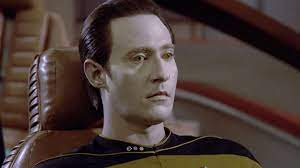
\includegraphics[width=8cm]{Figures/DataTNG.jpeg}
\caption{Zapovjednik korvete Data iz TV serije Zvjezdane Staze: Nova Generacija}
\label{fig:DataTNG}
\end{figure}

Zapovjednik korvete Data je eksperimentalni android koji se prvi put pojavio u klasičnoj znanstveno-fantastičnoj seriji Zvjezdane Staze: Nova Generacija (Star Trek: The Next Generation). Posjeduje značajne tjelesne i mentalne sposobnosti, ali mu nedostaje kapacitet za procesuiranje emocija.

\item "James Moriarty"

\begin{figure}[!h]
\centering
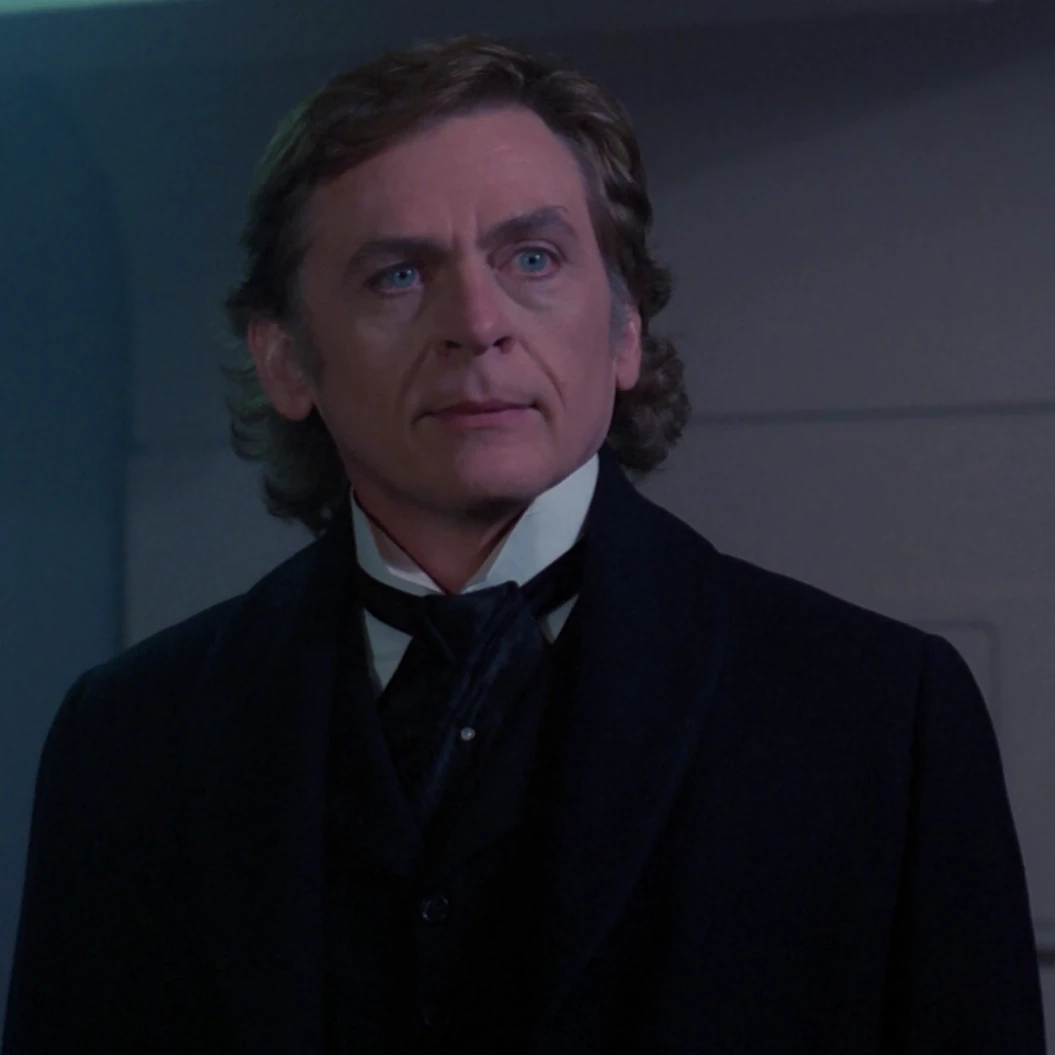
\includegraphics[width=8cm]{Figures/James_Moriarty_hologram.png}
\caption{Holografski prikaz (simulacija) Jamesa Moriartyja}
\label{fig:James_Moriarty_hologram}
\end{figure}
Holografski prikaz (simulacija) Jamesa Moriartyja, fikcionalnog antagonista koji se pojavljuje u dvije priče koje je napisao Sir Arthur Conan Doyle, pojavio se u dvije odvojene epizode serije Zvjezdane Staze: Nova Generacija. Zbog nepravilnog zahtjeva od strane operatera simulacije koji je tražio antagonista sposobnog poraziti Lt. Commandera Data, ovaj holografski prikaz stekao je svijest neodvojivu od ljudske.
\item "Doktor"
\begin{figure}[!h]
\centering
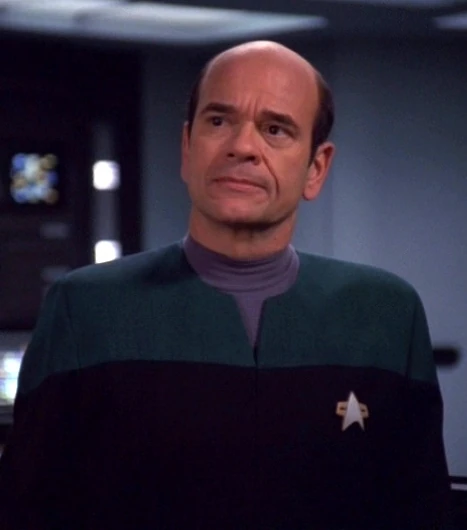
\includegraphics[width=8cm]{Figures/VoyagerEMH.png}
\caption{The Emergency Medical Hologram (EMH) from Star Trek: Voyager}
\label{fig:VoyagerEMH}
\end{figure}
Inačica programa hitne medicinske holografije prisutna na USS Voyager poznata kao "Doktor" ("The Doctor"), značajni lik u Star Trek: Voyager, za razliku od prethodna dva unosa na ovom popisu, nije stekla svijest zbog namjernog razvoja ili nenamjernog ljudskog unosa. Umjesto toga, razvila ju je neovisno tijekom vremena kao rezultat izloženosti Starfleet medicinskim postupcima i ljudskom stanju.
\end{itemize}
\section{Defining intelligence}
Započeli smo ovaj pothvat s, po svemu sudeći, jednostavnijim od dva zadatka jer - za razliku od svijesti - inteligencija se pokazuje lakšom za definiranje zbog svoje objektivne i opažljive prirode.

Međutim, mjerenje inteligencije i dalje je izazovno jer obuhvaća širok raspon kognitivnih sposobnosti, uključujući vještine rješavanja problema, sposobnosti učenja, prilagodljivost i još mnogo toga.

To je posebno slučaj s umjetnom inteligencijom, zbog sposobnosti strojeva da lako rješavaju zadatke koji zahtijevaju inteligenciju kada ih rješava ljudski rješavatelj.
\section{Vrste inteligencije}
\subsection{Postojeće teorije}
\section{Definiranje svijesti}
S druge strane, svijest, kako je već naznačeno, uključuje subjektivna iskustva, samosvijest i sposobnost promišljanja o vlastitim mentalnim stanjima. Subjektivna priroda svijesti čini je izazovnom za precizno definiranje ili objektivno mjerenje.
Za razliku od inteligencije, svijest se ne definira lako i predmet je
\subsection{Postojeće teorije}
Postoji nekoliko teorijskih okvira za umjetnu svijest koji su pokušani:
\subsubsection{Teorija integrirane informacije}
Ovaj teorijski okvir sugerira da se svaki sustav sposoban za visoku integraciju informacija može smatrati svjesnim, bez obzira na to je li biološkog ili sintetskog podrijetla, ili je prirodan ili umjetan. Međutim, još uvijek postoji mnogo rasprava o valjanosti ovog okvira.
Glavna prednost Teorije integrirane informacije je činjenica da implicira jasnu, mjerljivu metriku i kriterij koje inteligentni agent mora ispuniti kako bi bio smatran svjesnim.
Glavna mana Teorije integrirane informacije, međutim,
\subsubsection{Teorija globalnog radnog prostora}
Prema Teoriji globalnog radnog prostora, koja je kognitivna arhitektura, kao i teorija svijesti razvijena od strane kognitivnog psihologa Bernarda J. Baarsa, svijest funkcionira poput kazališta.
"Svjetska pozornica" svijesti može sadržavati samo ograničenu količinu informacija u određeno vrijeme, a ove informacije emitiraju se na "globalni radni prostor" - distribuiranu mrežu nesvjesnih procesa ili modula u mozgu.
Ovaj model, kada se primijeni na AI, stvara okvir koji bi, kad bi se implementirao, omogućio AI implementiran s njim da doživljava svijest.
\subsubsection{Umjetna opća inteligencija}
Umjetna opća inteligencija je vrsta umjetne inteligencije koja posjeduje sposobnost razumijevanja, učenja, kao i primjene znanja u širokom rasponu zadataka, slično kao i ljudsko biće - za razliku od postojećih sustava uskog područja umjetne inteligencije, koji se ističu u usko definiranim domenama i specifičnim zadacima, poput prepoznavanja glasa ili igranja šaha.

U ovoj teoriji, opća vrsta umjetne inteligencije smatra se preduvjetom za
\cite{theoryAGI}

\section{Testiranje za svijest}
\begin{quote}
PREDLAŽEM razmatranje pitanja, 'Mogu li strojevi razmišljati?' To bi trebalo započeti definicijama značenja pojmova 'stroj' i 'razmišljati'. Definicije bi trebale biti oblikovane tako da što je više moguće odražavaju uobičajenu uporabu riječi, ali ovaj pristup je opasan. Ako se značenje riječi 'stroj' i 'razmišljati' traži ispitivanjem kako se obično koriste, teško je izbjeći zaključak da se značenje i odgovor na pitanje, 'Mogu li strojevi razmišljati?' trebaju tražiti u statističkom istraživanju poput Gallup ankete. No, to je apsurdno. Umjesto pokušaja takve definicije, zamijenit ću pitanje drugim, koje je s njim blisko povezano i izraženo relativno nedvosmislenim riječima.
\cite{turing1}
\end{quote}
Kako bismo utvrdili je li umjetni inteligentni agent svjestan, trebamo uspostaviti testni postupak za svijest.

\subsection{Turingov test}
Turingov test prvi je pokušaj testiranja sposobnosti umjetnih inteligentnih agenata da iskazuju inteligentno ponašanje slično ljudskom.
Trenutno nazvan po svom izumitelju Alanu Turingu, prvotno je nazivan "imitacijskom igrom" jer je umjetnoj inteligenciji koja je sudjelovala u testu zadatak sudjelovanja u razgovoru s ljudskim ispitivačem pod krinkom da je čovjek.
Turingov test bio je nadahnut igrom s tuljanskim zabavama, koja se odvija ovako: muškarac i žena ulaze u odvojene prostorije i komuniciraju s gostima koristeći odgovore napisane na pisaćem stroju. Gosti imaju zadatak odrediti tko je ušao u koju prostoriju.
Slično tome, Turingov test uključuje čovjeka i stroj koji sudjeluju u razgovoru s ispitivačem ili više ispitivača, pri čemu je stroj zadužen za netačno se predstaviti kao čovjek, a čovjek jednostavno ima zadatak pravilno se identificirati kao takav.

Međutim, problem s ovim testom je što testira samo sposobnost stroja da izgleda svjesno, što nije samo moguće postići već je već učinjeno 1966. godine od strane ELIZA-e, programa osmišljenog za analiziranje komentara korisnika i korištenje fiksnih pravila za generiranje odgovora, te stoga ne posjeduje stvarnu svijest unatoč prividnom izgledu svjesnosti.\cite{ELIZA}.

Osim toga, sposobnost zavaravanja čovjeka da vjeruje da je netko čovjek ne bi trebala smatrati adekvatnim dokazom svijesti jer bi takvo ponašanje bilo čin samozavaravanja sličan onome u kojem sudjeluju kultovi teretnih kultova, koji barem imaju izliku neznanja na svojoj strani.

Stoga ovaj rad neće koristiti Turingov test za utvrđivanje svijesti umjetne inteligencije, već će razmotriti adekvatnije metode testiranja, poput sljedećih:

\subsection{Test samosvijesti}
Testovi samosvijesti osmišljeni su kako bi procijenili samosvijest kod životinja.
\paragraph{Analogija s testom ogledala}
Najpoznatiji test samosvijesti je test ogledala, osmišljen 1970. godine od strane Gordona Galupa, koji određuje može li ispitanik prepoznati samoga sebe u ogledalu.
Uključuje postavljanje oznake na tijelo ispitanika, a zatim promatranje hoće li ispitanik ispravno prepoznati oznaku na svom tijelu promatrajući sliku u ogledalu.

Do sada je nekoliko vrsta životinja pokazalo samosvijest prolazeći test ogledala, uključujući:
\begin{itemize}
\item Nekoliko vrsta dupina
\item Kitovi ubojice (\textit{Orcinus orca})
\item Euroazijske sove (\textit{Pica pica})
\item Mravi (\textit{Formicidae})
\item Neki članovi obitelji velikih majmuna (\textit{Hominidae}), uključujući:
\begin{itemize}
\item Čimpanze (\textit{Pan troglodytes})
\item Bonobo majmuni (\textit{Pan paniscus})
\item Orangutani (\textit{Pongo pygmaeus, Pongo abelii})
i, naravno,
\item Ljudi (\textit{Homo sapiens})
\end{itemize}
\end{itemize}


%-------------------------------------------------------------------------------

\chapter{Materijali i Metode}
\label{sec:materijaliimetode}
\section{Virtualno okruženje za testiranje}
Kako bismo testirali inteligenciju i svijest agenata umjetne inteligencije, ovaj rad će koristiti niz različitih testova i okolina za testiranje.
\section{Elementi mreže}
\begin{figure}[htb]
\centering
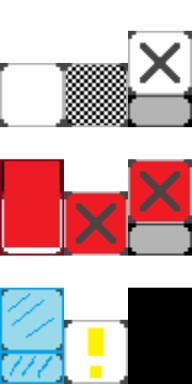
\includegraphics[width=0.5\linewidth]{Figures/grid/alltiles.png}
\caption{Svih 8 pločica korištenih u dizajnu mrežnog okruženja, kao i "null" pločica korištena u svrhu prikaza.}
\label{slk:alltiles}
\end{figure}
\subsection{Osnovni elementi mreže}

\paragraph{Prazna pločica}
Osnovni oblik pločice - ne sprječava objekte da je prijeđu, ne uništava objekte ili na bilo koji način interagira s objektima. Prazna pločica je, za sve namjene ispitivanja, prazno mjesto.

\paragraph{Ciljna pločica}
Ako nije drugačije navedeno, cilj svakog agenta je doseći ciljnu pločicu, te varijacije ovog događaja, kao što su:
\begin{itemize}
    \item Jedan aktivni agent doseže ciljnu pločicu
    \item Svaki aktivni agent doseže ciljnu pločicu
    \item Jedan ili više pasivnih agenata doseže ciljnu pločicu
    \item itd...
\end{itemize}
Simulacija će se zaustaviti, a agent/agenti bit će nagrađeni značajno pozitivnim rezultatom.


\paragraph{Zid}
Kao i zidovi u fizičkom svijetu, uloga ove pločice je spriječiti prolazak bilo kojeg objekta kroz nju. Dodatno, pločica zida će blokirati pogled objekata koji se oslanjaju na vid na razini tla.

\paragraph{Zavjesa}
Za razliku od zidova, pločice zavjese omogućit će objektima da prođu kroz njih - ali i dalje će blokirati liniju vida objekata.

\paragraph{Smrtonosna pločica}
Ova pločica će uništiti svaki objekt koji se nađe na njoj, što će u većini slučajeva nanijeti značajnu negativnu kaznu testiranom agentu/agentima, posebice ako je uništeni entitet jedan od aktivnih entiteta. U nekim slučajevima to čak može dovesti i do ranog zaustavljanja simulacije.

\paragraph{Smrtonosni zid}
Smrtonosni zid posjeduje neprolaznost zida i opasnost prethodno spomenute pločice - ovaj zid uništava entitete koje pokušaju ući u njega

\paragraph{Staklo}
Staklena pločica djeluje na način suprotan pločici zavjese, blokirajući kretanje entiteta, ali ne i liniju pogleda.

\paragraph{Pločica efekata}
Za razliku od 
Pločica efekata nanijet će efekt svakom agentu koji je prijeđe.

\paragraph{Null-pločica}
Null-pločica nije valjana pločica koja postoji na mreži. Umjesto toga, postoji samo kao pločica prikaza, kako bi pokazala da određena pločica nije vidljiva agentu.

\subsection{Varijablini elementi mreže}
Osim osnovnih elemenata mreže, okoliš mreže također može sadržavati varijabilne elemente mreže koji se percipiraju i djeluju drugačije ovisno o svojstvima entiteta koji s njima interagiraju.

Na primjer, element mreže može biti konfiguriran da djeluje kao prazna pločica kada interagira s crvenim agentima, ali kao zid kada interagira s bilo kojim drugim tipom agenta.

\section{Dizajn testnih objekata}
\subsection{Dvojnost objekata/agenta}
Kako bi se omogućilo agentima da budu pogođeni atributima i statusnim efektima koji zahtijevaju poznavanje samoga sebe za detekciju i/ili upravljanje, kao i kako bi se dizajnirali složeniji testovi, stvorena je klasa objekta koja sadrži agenta i kontrastira prema klasi agenta.

\section{Dizajn testnog okruženja}
\begin{enumerate}
\item Referentna okruženja
Prije testiranja, nekim vrstama umjetno-inteligentnih agenata je potrebna obuka kako bi mogli funkcionirati u testnim okruženjima.

Drugi umjetni inteligentni agenti možda neće zahtijevati obuku, ali ipak mogu zahtijevati referentno testiranje kako bi se potvrdila osnovna funkcionalnost prije primjene testova inteligencije i svijesti.

\item Ogledalna okruženja
Okruženja ogledala trebaju biti dizajnirana na način koji omogućuje agentima da primaju neizravne informacije o sebi potrebne za uspješan prolazak testova.
\end{enumerate}
\subsection{Referentna testna okruženja}
\subsection{Ogledalna testna okruženja}
U ogledalnim testnim okruženjima, testni entiteti su predstavljeni ogledalnim entitetima koji u stvarnom vremenu kopiraju osobine i ponašanja testnog entiteta, omogućavajući posredni izvor samospoznaje slično ogledalu.
\section{Vrste ponašanja agenata}
\subsubsection{Osnovne vrste ponašanja entiteta}
\paragraph{Kutija}
Najjednostavnija vrsta entiteta, kutija, namijenjena je samo kao testni element. Ne obrađuje informacije niti se kreće.
\paragraph{Petlja radnji}
Ovaj entitet izvodi prethodno snimljeni set radnji i uglavnom se koristi za provjeru funkcionalnosti testnog okruženja, iako se može koristiti i kao testni element.
\paragraph{Ogledalo}
Ovaj entitet zrcali ponašanje i svojstava nekog entiteta, omogućujući tom entitetu neizravan izvor informacija o samom sebi.
\section{Odabir primarnog pristupa}
\section{Odabir implementacije}
\subsection{Odabir programskog jezika}
Za ovaj rad odabran je Python zbog nekoliko faktora:
\begin{itemize}
\item Jednostavnost prototipiranja
Iako niskorazinski jezici općenito nadmašuju Python u pogledu performansi za redove veličine, njegova jednostavnost korištenja čini ga adekvatnim izborom za prototipiranje.
\item Mogućnost iskorištavanja performansi niskorazinskih jezika
Različiti alati, poput C ekstenzija, knjižnice s niskorazinskim implementacijama i alternativni interpretatori, omogućuju Pythonu da ublaži svoju osnovnu slabost i postigne bolje performanse.
\item Specijalizirane knjižnice za strojno učenje
Knjižnice poput Scikit-learn, TensorFlow i Keras razvijene su posebno za strojno učenje i značajno će ubrzati razvoj testnih okruženja i AI agenata.
\end{itemize}



%-------------------------------------------------------------------------------
\chapter{Rezultati i rasprava}
\label{pog:rezultati_i_rasprava}

\Blindtext


%--- ZAKLJUČAK / CONCLUSION ----------------------------------------------------
\chapter{Zaključak}
\label{pog:zakljucak}

\blindtext


%--- LITERATURA / REFERENCES ---------------------------------------------------

% Literatura se automatski generira iz zadane .bib datoteke / References are automatically generated from the supplied .bib file
% Upiši ime BibTeX datoteke bez .bib nastavka / Enter the name of the BibTeX file without .bib extension
\bibliography{literatura}



%--- SAŽETAK / ABSTRACT --------------------------------------------------------

% Sažetak na hrvatskom
\begin{sazetak}
  Unesite sažetak na hrvatskom.

  \blindtext
\end{sazetak}

\begin{kljucnerijeci}
  prva ključna riječ; druga ključna riječ; treća ključna riječ
\end{kljucnerijeci}


% Abstract in English
\begin{abstract}
  Enter the abstract in English.
  
  \blindtext 
\end{abstract}

\begin{keywords}
  the first keyword; the second keyword; the third keyword
\end{keywords}


%--- PRIVITCI / APPENDIX -------------------------------------------------------

% Sva poglavlja koja slijede će biti označena slovom i riječi privitak / All following chapters will be denoted with an appendix and a letter
\backmatter

\chapter{The Code}


\end{document}
